\section{Sequence diagrams}\label{app:sequence-diagrams}

\begin{figure}[!hpt]
    \centering
    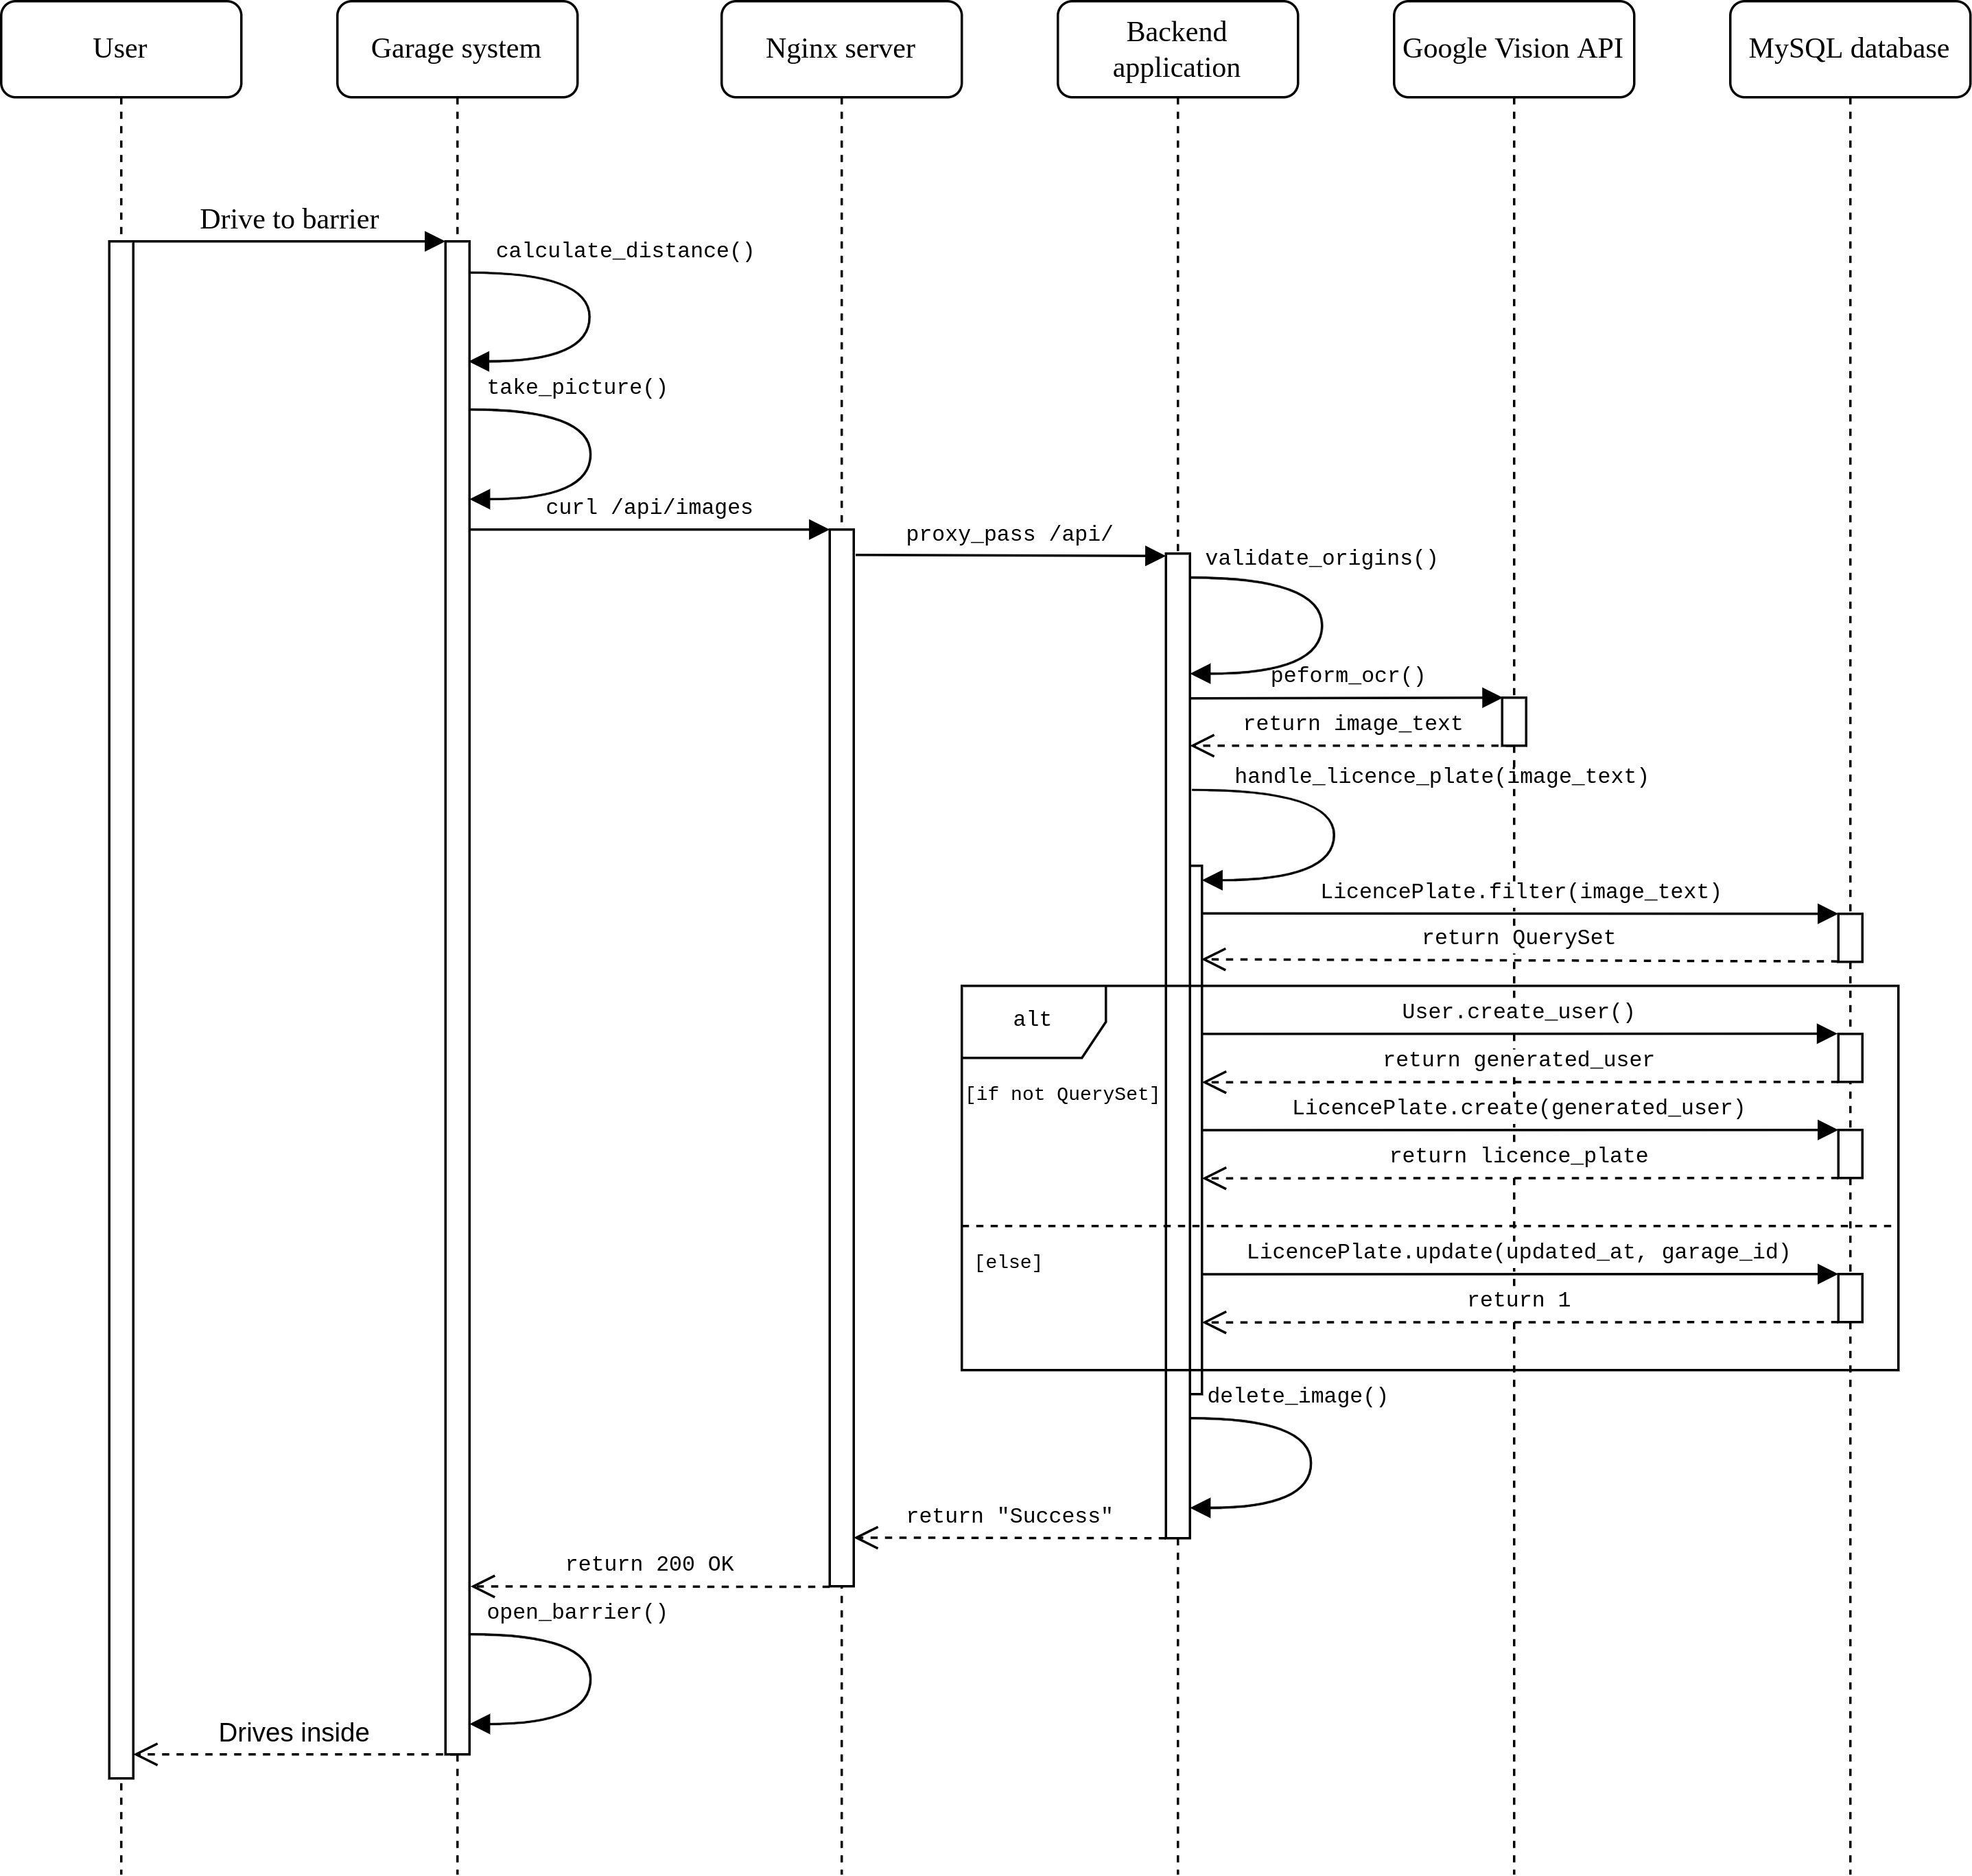
\includegraphics[width=16cm]{images/sequence_diagrams/sequence_diagram_licence_plate.drawio.png}
    \caption{Sequence diagram of the licence plate registration in the local garage system.}
    \label{fig:sequence-diagram-licence-plate}
\end{figure}

\begin{figure}[!hpt]
    \centering
    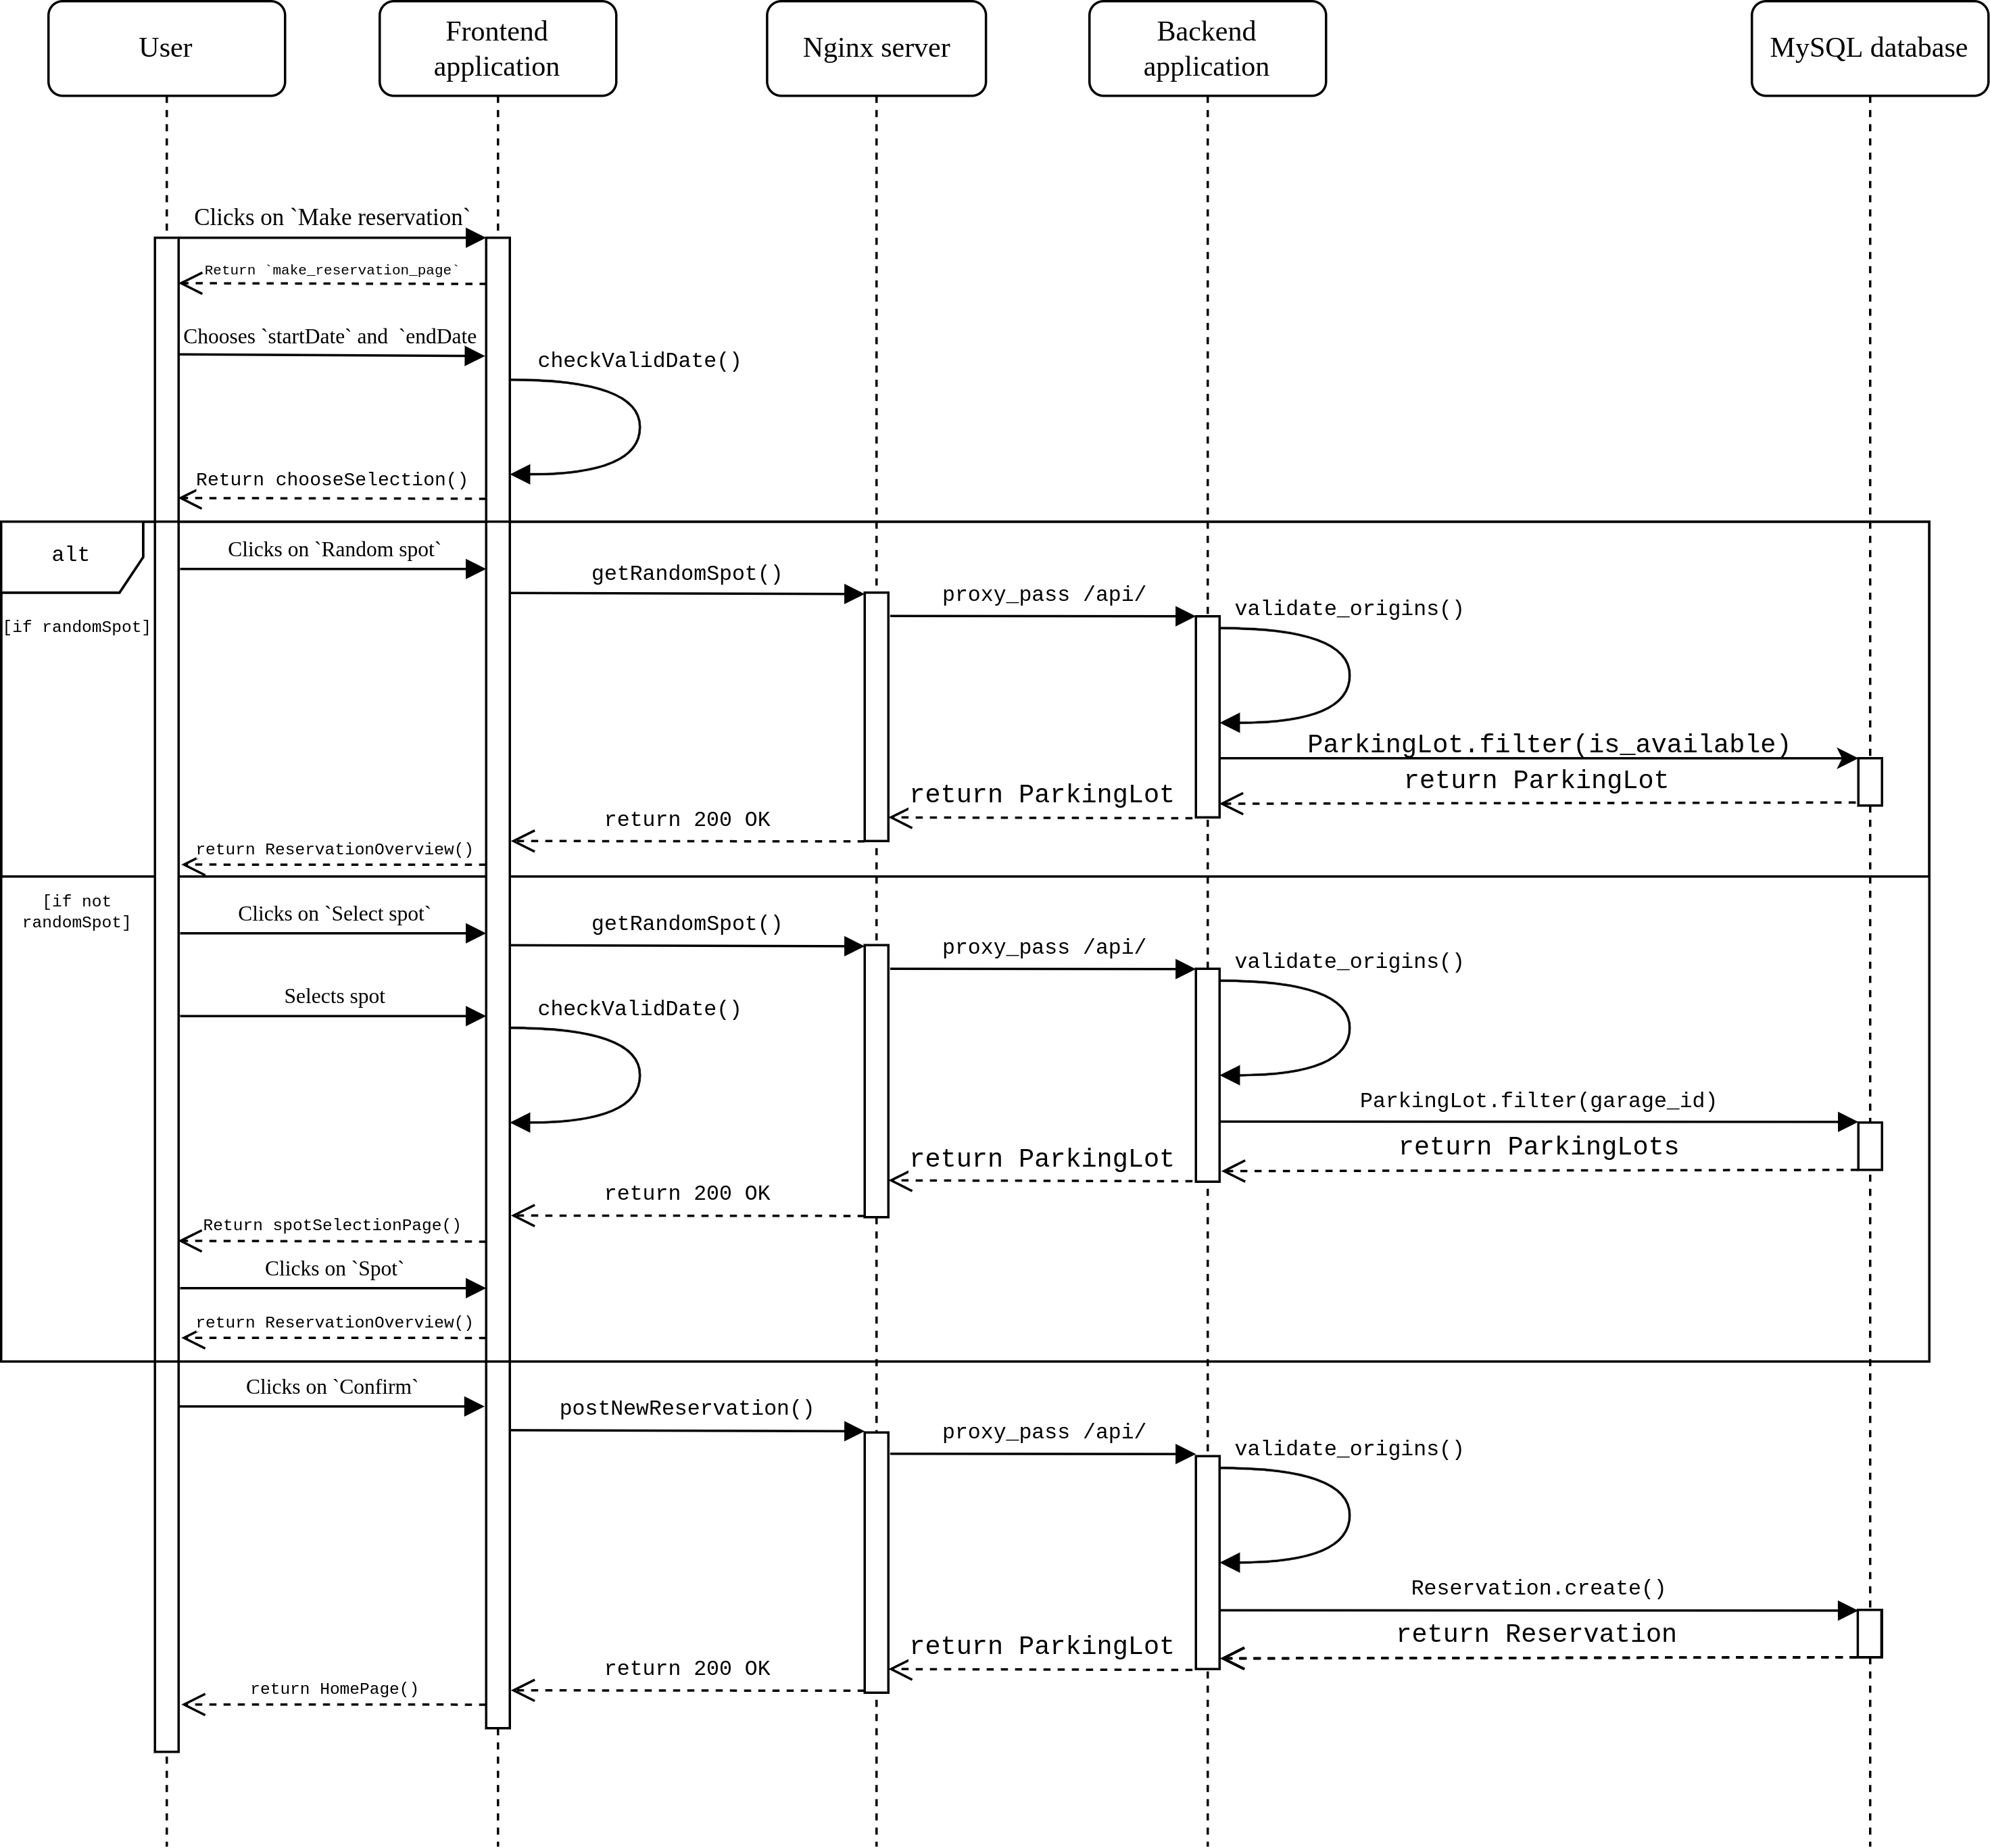
\includegraphics[width=16cm]{images/sequence_diagrams/sequence_diagram_reservation.drawio.png}
    \caption{Sequence diagram of the reservation flow.}
    \label{fig:sequence-diagram-reservation}
\end{figure}
\clearpage

\begin{figure}[!hpt]
    \centering
    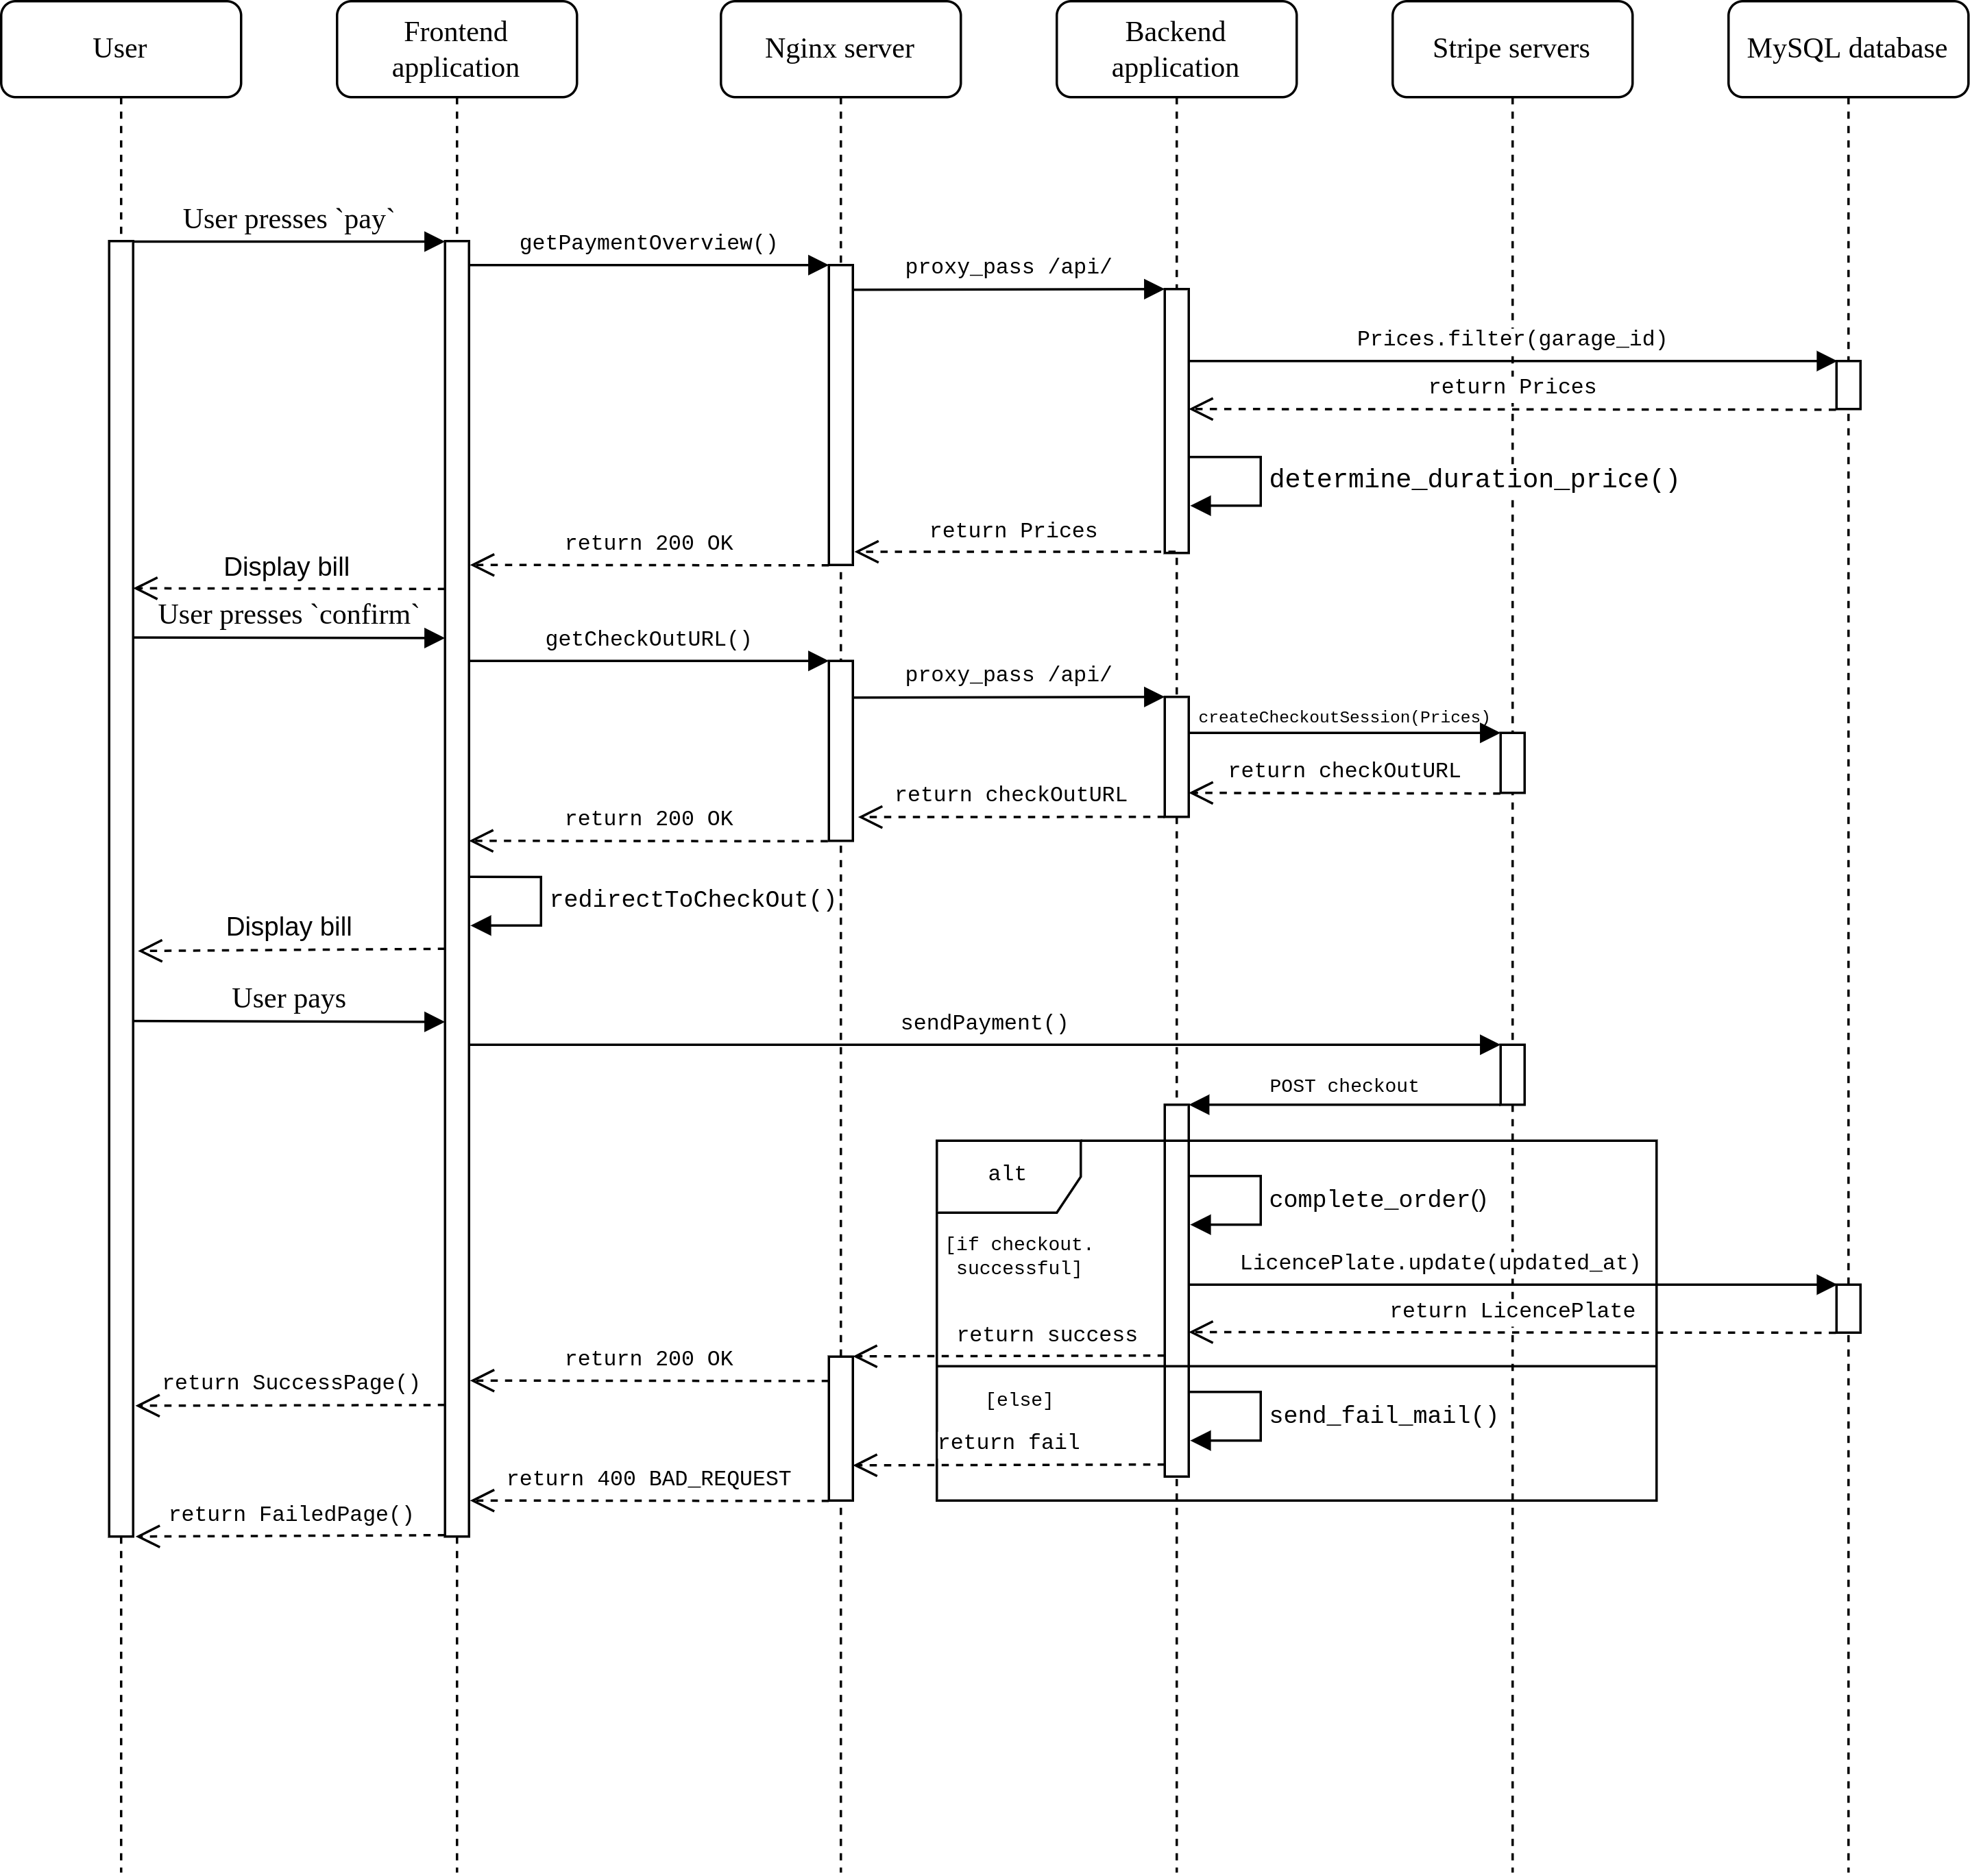
\includegraphics[width=16cm]{images/sequence_diagrams/sequence_diagram_manual_payment.png}
    \caption[Sequence diagram of the manual payment]{Sequence diagram of a manual payment. Note that this represents a payment without errors.}
    \label{fig:manual-payment}
\end{figure}

\begin{figure}[!hpt]
    \centering
    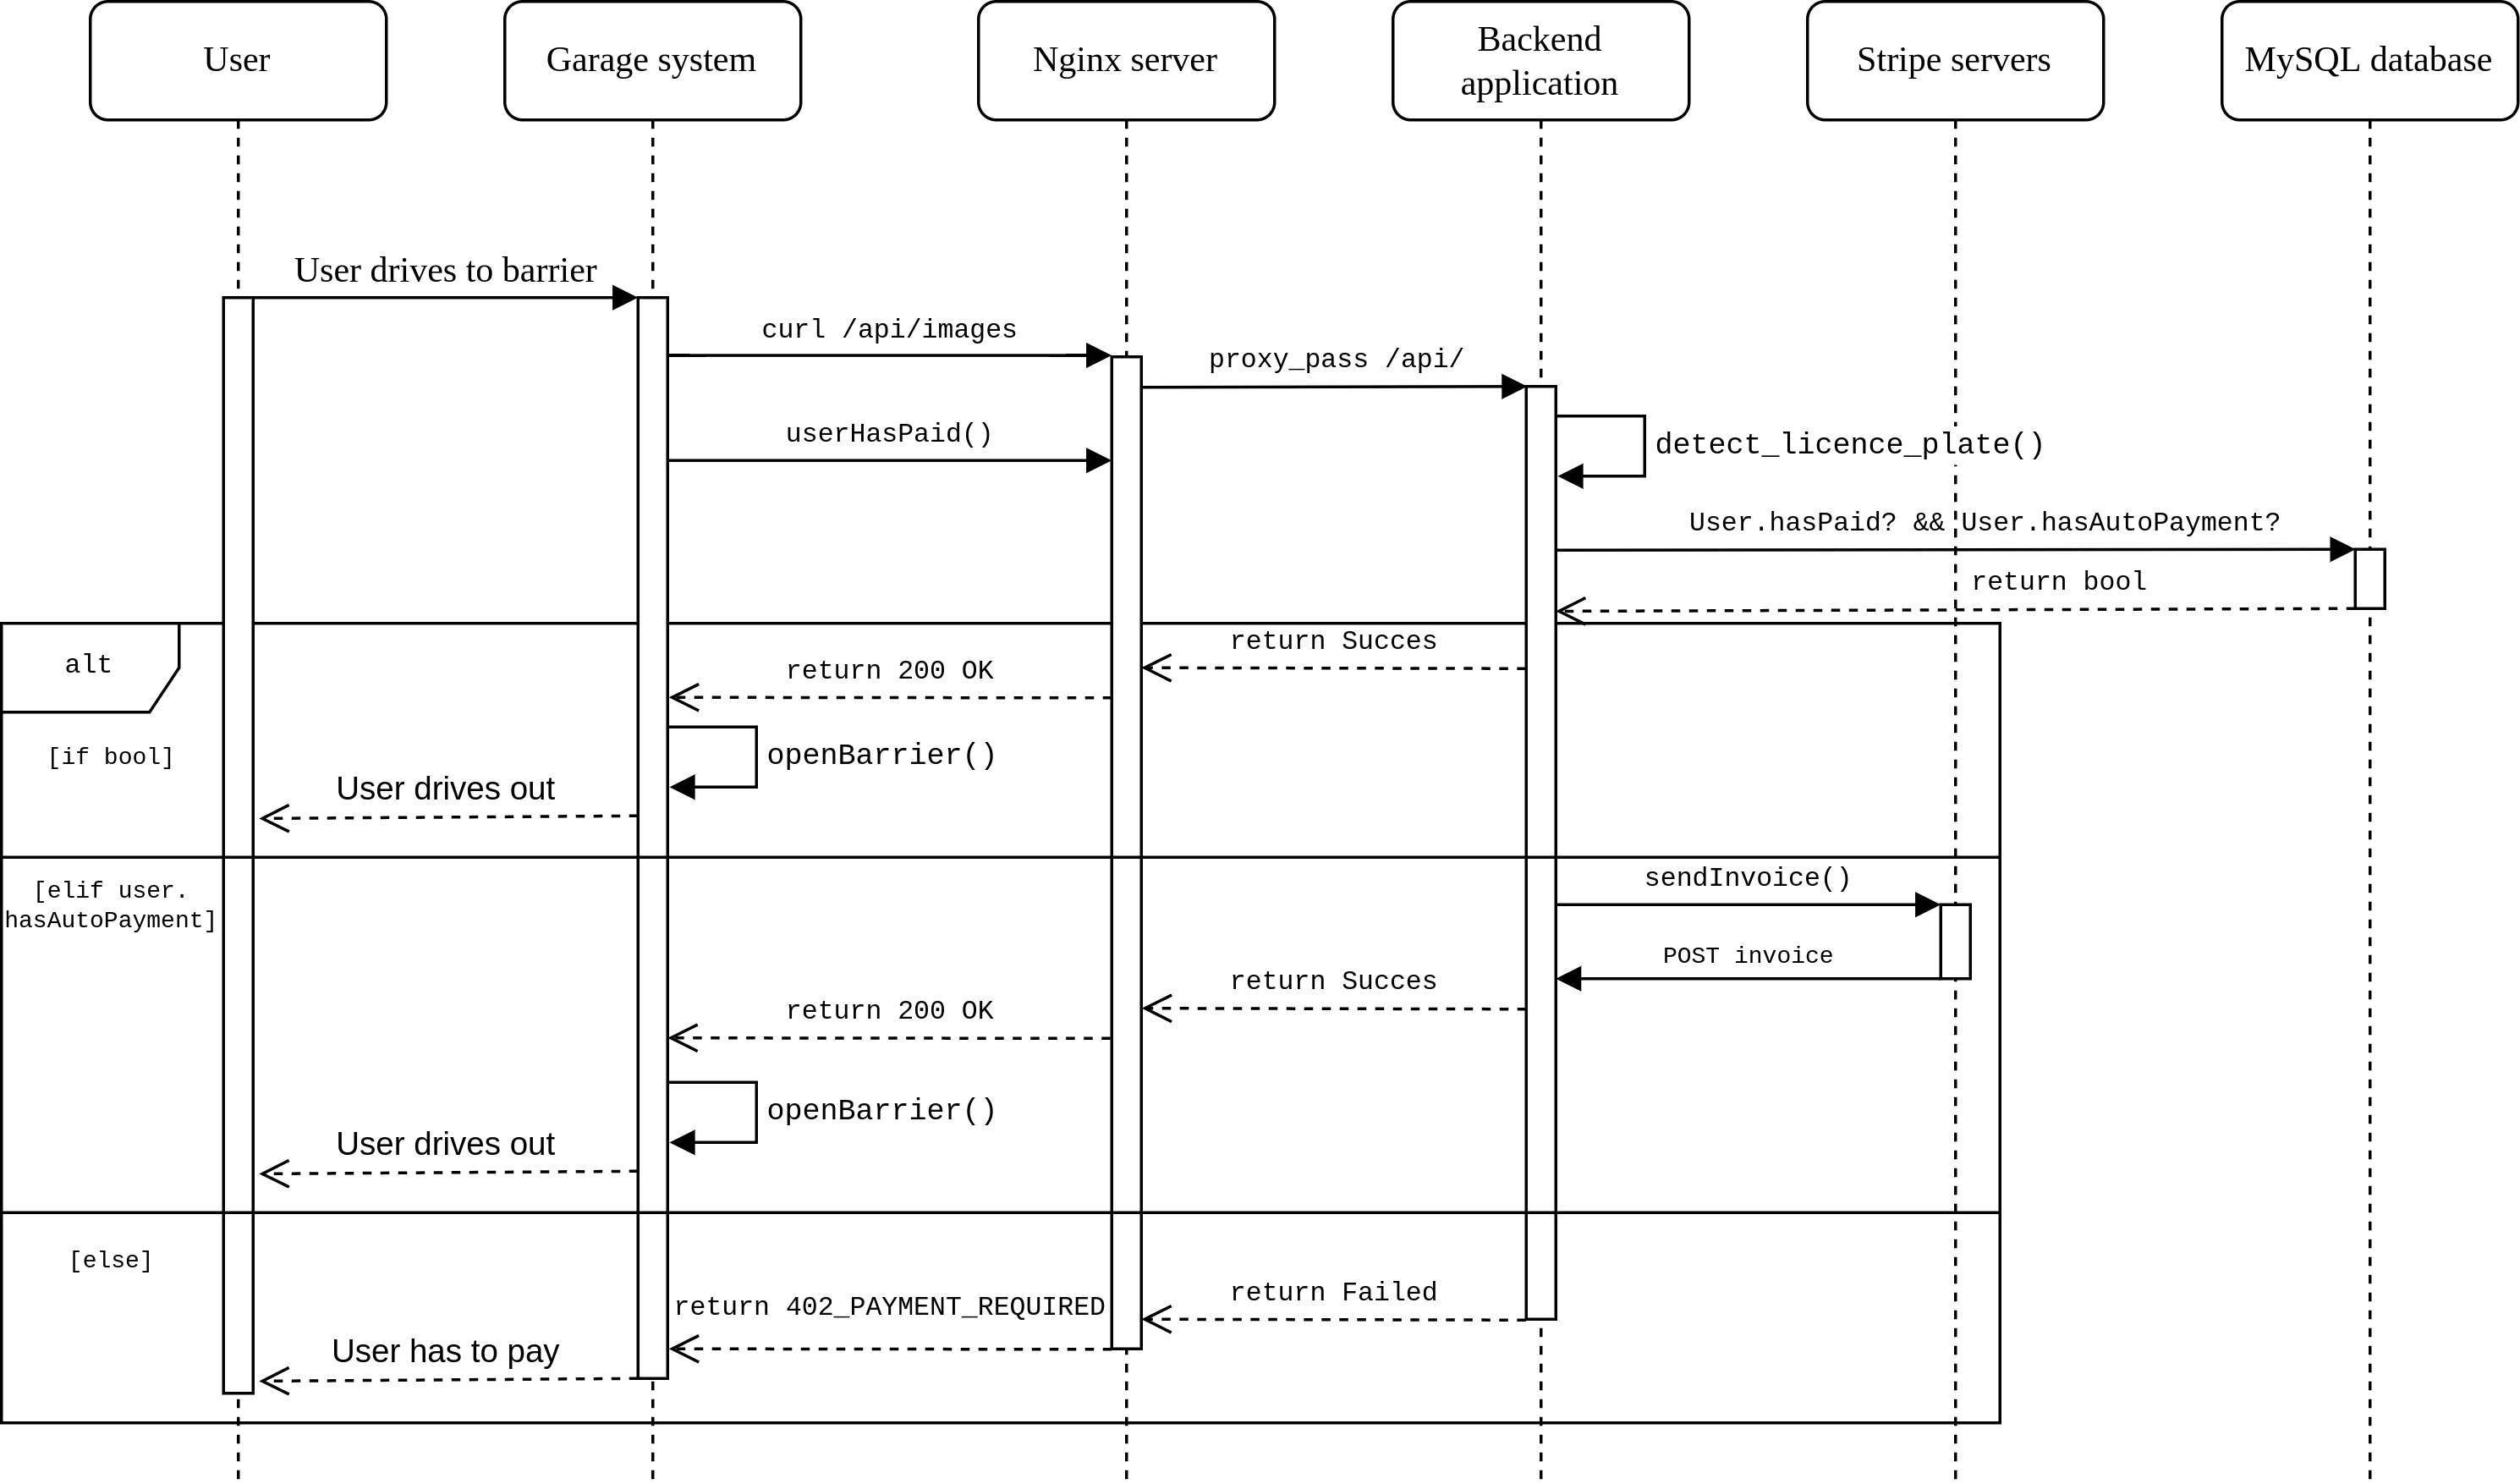
\includegraphics[width=16cm]{images/sequence_diagrams/sequence_diagram-automatic_payment.jpg}
    \caption[Sequence diagram of the automatic payment]{Sequence diagram of a automatic payment. Note that this represents a payment without errors. The \texttt{detect-licence-plate()}-function is implemented with the sequence diagram of Figure 19.}
    \label{fig:automatic-payment}
\end{figure}


\clearpage